\documentclass[english,
    %BCOR%Bindungskorrektur,
    ]{WissTemplate}
    %\PassOptionsToPackage{usenames,dvipsnames}{xcolor}
\usepackage{
    datetime,
    ulem,
    tikz, %grafiken generieren
    varwidth, %anpassen von seitengrößen
    enumitem,
    longtable,
    pgfplots, %diagramme
    caption, %tabbellen beschreibungen
    url,
    listings, %code blöcke
    hyperref %links
    }
\usetikzlibrary{positioning,shapes,shadows,arrows, arrows.meta, calc,
    automata, petri %petri netze
    }
%\usepackage[a4paper,left=27mm,right=27mm, top=1cm, bottom=2cm]{geometry}

\renewcommand{\name}{Tom Meyer}
\renewcommand{\strasse}{Thomas-Müntzer-Platz 64}
\renewcommand{\stadt}{18057 Rostock}
\renewcommand{\matrikel}{Matrikel-Nr.: 8200839}
\renewcommand{\course}{Informatik}
\renewcommand{\betreuer}{Prof. Dr. Karsten Wolf}
\renewcommand{\Titel}{Eine Petrinetzsemantik für Rust}
\renewcommand{\Type}{Masterarbeit } %Bachelorarbeit, Projektarbeit, Literaturarbeit, etc.

\definecolor{verylightgray}{rgb}{0.95,0.95,0.95}
\tolerance=1000 
\hyphenpenalty=1000

\begin{document}

\hypersetup{
	pdftitle   = {\Titel},
	pdfauthor  = {\name, \matrikel},
	pdfsubject = {\Type betreut von \betreuer}
}

\begin{titlepage}
	\newlength{\BCORoffset}
	\ifdefined\BCOR
		\setlength{\BCORoffset}{0.5cm}
	\else
		\setlength{\BCORoffset}{0cm}
	\fi
	\linespread{1.2} % 1,5facher Zeilenabstand
	\begin{tikzpicture}[remember picture,overlay, anchor = west]

		\coordinate (d) at ([yshift=-6cm, xshift=-2cm+\BCORoffset] current page.north east);
		\coordinate (c) at ([yshift=-6cm, xshift=2cm+\BCORoffset] current page.north west);
		\coordinate (b) at ([yshift=2.25cm, xshift=-2cm+\BCORoffset] current page.south east);
		\coordinate (a) at ([yshift=2.25cm, xshift=2cm+\BCORoffset] current page.south west);
		\coordinate (middle) at ([yshift=-6cm, xshift=\paperwidth/2+\BCORoffset] current page.north west);
		\draw[line width=2,rounded corners=10pt,uniblau] (a) -- (c) -- (d) -- (b);
		
		\node[anchor=west,inner sep=0,outer sep=0] (logo) at ([yshift=-3cm, xshift=2cm+\BCORoffset] current page.north west) {
			
\includegraphics[width=115mm]{Icons/UNI-Logo_Siegel_4c_115mm}
		};
		
		\node[fill=uniblau,draw=uniblau,line width=2,anchor=north,minimum height=2.25cm, minimum width=\paperwidth-4cm,text=white,font=\small,text width=\paperwidth-4.5cm] (names)
		at ([yshift=2.25cm,xshift=\BCORoffset]current page.south) {
			UNIVERSITÄT ROSTOCK \textbar \ FAKULTÄT FÜR INFORMATIK UND ELEKTROTECHNIK\\
			Lehrstuhl für Theoretische Informatik\\
			Albert-Einstein-Straße 22, 18059 Rostock \textbar \ Tel: +49 381 498 7641	
		};
		
		\node[font=\Huge\bfseries,anchor=center,] (typenode) at ([yshift=-3cm] middle) {\Type};
		
		\node[font=\LARGE\bfseries,anchor=center,] (titelnode) at ([yshift=-2.5cm] typenode) {\Titel};
		
		\node[font=\large,anchor=center,text width=\paperwidth-4.5cm,align=center] (authornode) at ([yshift=-3.5cm] titelnode) {
			\textsc{Vorgelegt von}:\\ \bfseries\name\\\mdseries \textsc{\matrikel}
		};
		
		\node[font=\large,anchor=center,text width=\paperwidth-4.5cm,align=center] (abgabenode) at ([yshift=-4.5cm] authornode) {
			\textsc{Eingereicht am:}\\ datum
		};
		
		\node[font=\large,anchor=center,text width=\paperwidth-4.5cm,align=center] (supervisornode) at ([yshift=-4.0cm] abgabenode) {
			\textsc{Betreuer:}\\\betreuer
		};
	\end{tikzpicture}
\end{titlepage}
\restoregeometry

\frontmatter
% !TEX root = ../main.tex
% TODO: Schau dir nochmal ein paar Paper abstracts an.
% Du solltest vorher noch einen Satz zur Motivation schreiben, und vor den letzten Satz noch einen Satz zu Ergebnissen schreiben.
\section*{Eine Petrinetzsemantik für Rust}
Es wird ein allgemeiner Ansatz gezeigt Rustprogramme in ein Petrinetzmodel zu überführen.
Die Übersetzung eines Beispielprogramms wird als Eingabe in einem Model-Checker verwendet um einen Deadlock zu finden, der durch mehrfaches blockieren eines Mutex verursacht wir.
Anschließend werden einige Vorschläge zur Verbesserung der gezeigten Übersetzung diskutiert.

\section*{A Petri-Net semantics for Rust}
We show a general approach to translate a Rust program into a Petri-Net model.
An example program is used as input for a model checker to find a contained deadlock.
The deadlock is caused by locking a mutex multiple times.
In the last part of this work we discuss how our approach can be improved further.

\vfill

\begin{tabular}{ll}
	\bfseries Betreuer: & \parbox[t]{10cm}{\betreuer }\vspace{5mm} \\
	\bfseries Tag der Ausgabe: & 27.09.2019 \\
	\bfseries Tag der Abgabe: & 13.03.2020 \\
\end{tabular}

\tableofcontents
\newpage
\markright{\nomname}
\printnomenclature
%\addcontentsline{toc}{chapter}{\nomname}
% Abbildungsverzeichnis
%\newpage
%\addcontentsline{toc}{chapter}{\listfigurename}
%\addcontentsline{toc}{chapter}{Abbildungsverzeichnis}
%\listoffigures
%\newpage
% Tabellenverzeichnis
%\addcontentsline{toc}{chapter}{\listtablename}
%\listoftables
\mainmatter

% !TEX root = ../main.tex
\chapter{Introduction}
\label{introduction}
% !TEX root = ../main.tex
\chapter{Background and related work}
\section{Rust}
\label{rel_rust}
\begin{verbatim}
- rust empowers bla bla \cite{}
- low level with high level abstractions
- small runtime
- no garbage collection
- controlled memory access
  - reduced expressiveness in exchange for increased memory safety
  - features to tackle memory safety issues
  - borrow checker
  - no data races etc
- fast vs safe vs compile time effort \cite{}
- deadlocks are considered safe in rust terms \cite{}
\end{verbatim}

\section{Compiler}%?????
????


\section{Parallel Programs}
\label{rel_para}
\begin{verbatim}
- the problem with parallel programs
  - need to communicate data
    - messages
    - shared memory
  - data needs to be 
    - consistent 
    - synchronized (wait for each other)
    - up to date
  - deadlocks can easily be introduced with 
    synchronisation flaws \cite{}
- what are deadlocks
  - synchronisation
  - mutex/semaphore
  - threads
  - dining philosophers
- rust and parallel programs
- how can deadlocks be introduced in rust
  - rust and deadlocks -> considered safe code
\end{verbatim}

\section{Model Checking}
\label{rel_mc}
\begin{verbatim}
- tests vs Model Checking
  - tests 
    - only work for specific cases\cite{}
    - done by program execution
  - Model Checking 
    - works in the general case\cite{}
    - done by program analysis
- different approaches (BDDs etc.)
- petri nets!!
\end{verbatim}

\subsection{Petri-Nets}
\label{rel_petri}
\begin{verbatim}
- 
\end{verbatim}

\subsection{CTL*}
\label{rel_ctl}
\begin{verbatim}
- 
\end{verbatim}

\begin{verbatim}
  - other verification implementations
    - (verification by language?)
      - functional programming invariants?
      - prolog invariants?
      - languages with verification methods in its design?
    - c verification
      - valgrind?
    - rust verification
  - petri net verification
    - bpel
\end{verbatim}
% !TEX root = ../main.tex


\chapter{Approach}
After we learned the underlying concepts, we can go on with the actual task.

In this chapter it is shown how the initial rust code is translated and analysed.
We will see that the rust compiler has interfaces that we can use to reduce our effort,
and that it creates an intermediate representation that fits our needs nicely.
We will work out a translation for the elements of this intermediate representation, 
and discuss the format that we will translate into.
Finally we will discuss how we can use a model checker to find deadlocks in some simple test programs.
%TODO: überleitungssatz?

\section{Rust Compiler}
\label{app_rust}
There are basically two options to translate rust into Petri-Nets:
\begin{enumerate}
    \item write an own translator or,
    \item use something existing.
\end{enumerate}
Writing an own translator means total control over the process.
Features can be added iteratively as needed and data structures can be designed efficiently for this special perpose.
However, this would result in a new compiler for rust which eventually has to cover every language feature;
Including some difficult ones like macro expansion and generics.
Features that someone already implemented, spending a fair amount of thought in the process;
Backed by a large community;
Over several years.
Resulting in a compiler that is openly available under an open source license\cite{rustc}, with a maintained documentation\cite{rustc-guide}\cite{rustc-doc}.
And even though learning how this complex compiler works, and where to find the relevant parts for this project is also difficult, it seems to be time worth spend if we are able to skip learning and implementing difficult features.
For this reason this project is based on the rust compiler `rustc'.
So lets see how its basic structure looks like.

The rust compiler does have several phases and a variety of intermediate representations \cite[Chapter 2.1]{rustc-guide}:
\begin{enumerate}
    \item In the first phase rust source files are parsed to an abstract syntax tree (\textbf{AST}) that matches the original syntax closely.
    \item In the second phase implicit information is expanded. This includes for example macros and identifier names.
    \item Phase three lowers the AST to a simpler form called high-level intermediate representation or \textbf{HIR}.
    The HIR still is quite similar to normal rust syntax but some structures are normalised so that code analysis is easier. 
    For example for loops are rewritten to simple endless loops with break conditions.
    \item The fourth phase executes some static analysis on the HIR.
    Things like type checking and encapsulation verification is done on this representation.
    \item Another representation is generated in phase five: the mid-level intermediate representation (\textbf{MIR}).
    Now we leaving the tree structure and switching to a graph.
    MIR is based on a control-flow graph \cite{} and language features are reduced to a minimum.
    There is only one type of loop and branches respectively (only gotos instead of ifs or pattern matching).
    Additional static analysis is done on the mir level,
    like rusts borrow checking, as well as further optimization.
    \item Phase six lowers the MIR to the rust independant LLVM\cite{} intermediate representation.
    LLVM IR is a low level representation that is close to assembly language.
    Optimization for this representation can now be done for the code resulting in several object files.
    \item In the last phase the object files are linked into a complete binary executable.
\end{enumerate}
But wich phase is best to intercept to translate the current intermediate representation into petri nets?

\section{Interception strategie}
\label{app_intercept}
After deciding to use the rust compiler as basis for this work, we need to determine the phase we want to intercept the default compilation to translate to our own target.
A suitable location makes use of the most possible compiler features with the least amount of translation effort.

We want to skip basic features like name resolution as we need this feature ourselfs and surely won't improve it by a reimplementation.
Also code generation, including macro and generics expansion, should be handled by the compiler.
They just produce more rust code that we will treat anyway.
But after expansion, no code generation syntax will remain and we can simply ignore this feature.

More optional for our use are the static analysis features like type checking and borrow checking.
Though, we want to use their assumption, we do not depend on them actually being checked, since nobody will ever run a rust program that did not go through the complete compilation process.
So it is quite safe to assume that nobody will do model checking on a program that won't compile.
However, we still can enforce those invariants if we run the static analisis anyway and abort on errors.
This prevents time consuming runs for programs that cannot be build.

A compiler feature that \textit{can} greatly ease our effort is the lowering of the representation.
After all that means that several high level language features are reduced to less low level features.
Which in turn means less features we have to cover with our implementation.
We don't want to go to low though, since lower representations might prevent us from exploiting assumptions that are hidden in the translation process.
We also probably want to avoid a machine dependant representation.
To verify generic rust programs and not the peculiarities of a single machine.
This might be debateable though.

Lastly we want to make use of all optimizations we can.
Especially optimizations that reduce the code (and resulting net) size.
So features like constant propagation and dead code elimination would be nice to have to reduce the limit of state explosion.
At least a little bit.

Looking back an the rust compiler phases with those thoughts in mind, the seemingly best place we can intercept is between phase five and six.
After borrow checking and optimizations on the MIR.
Here, all code was expended, all rust specific static analisis and optimization was done and all unnecessary language features where reduced to a minimal set of instructions.
And since MIR is a graph representation as well as petri nets, a mapping should be relatively straight forward.
More so if we consider that MIR represents control flow quite closely as petri nets do.
Also we avoid the still lower level and rust independent LLVM IR and the machine dependent object files. 

\section{Mid-level Intermediate Representation (MIR)}
\label{app_mir}
%TODO: examples examples examples

Now where we pinned down MIR as the intermediate representation to use, it is helpful to understand how it is structured.

\begin{figure}
    \centering
    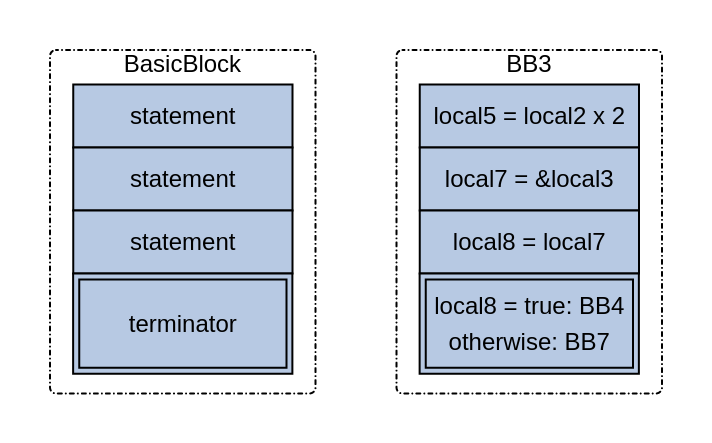
\includegraphics[width=.7\textwidth]{../diagrams/BasicBlock.png}
    \caption{
        Structure of a basic block. 
        Several chained statements with a single trailing terminator.
        The terminator can redirect control flow to other basic blocks.
        In this example BB3 branches to BB4 or BB7 depending on the value of local8
        }
    \label{mir_bb}
\end{figure}

As mentioned before, MIR is derived from control flow graphs\cite[chapter 2.17]{rustc-guide}.
It consists of several \textbf{basic blocks} which are interconnected with directed edges.
Each basic block consist of any amount of non branching \textbf{statements} and a single -- possibly branching -- \textbf{terminator}.
All statements in a single basic block are executed sequentially.
Between those, no branching can occur in or out.
Only terminators can redirect the control flow.
They are the ones that represents conditional execution (i.e. if-then-else constructs) or jumps to other basic blocks (including loops).

% \lstset{language=C++,caption={Basic implementation of a spinlock with compare and swap},label=CASIMPL, frame=none, stepnumber=5, backgroundcolor=\color{verylightgray}}
% \begin{lstlisting}
% #include <atomic>

% enum LOCK{
%     LOCKED,
%     UNLOCKED
% };

% static inline void waitAndLock(std::atomic<bool>* lock){
%     bool expected = UNLOCKED;
%     while (!lock->compare_exchange_weak(expected,LOCKED)){
%         expected = UNLOCKED;
%     }
% }

% static inline void waitForUnlock(std::atomic<bool>* lock){
%     while (lock->load() != UNLOCKED){
%         continue;
%     }
% }

% static inline void lock(std::atomic<bool>* lock){
%     lock->store(LOCKED);
% }

% static inline void unlock(std::atomic<bool>* lock){
%     lock->store(UNLOCKED);
% }
% \end{lstlisting}

Data in MIR is represented as \textbf{locals} and \textbf{places} (not to be confused with petri-net places).
Places represent any kind of memory location, whereas locations are conceptually located on the stack.
This means that a location can also be represented as a place, but places are not necessarily locations.
Statements work on these data representations.
The most prominent type of statement is an assignment that assigns an \textbf{rvalue} derived from an expression to a memory location -- meaning a place.
Also based on the data terminators can direct control flow.
Which branch the program takes might depend on the value a place currently holds.

\begin{figure}
    \centering
    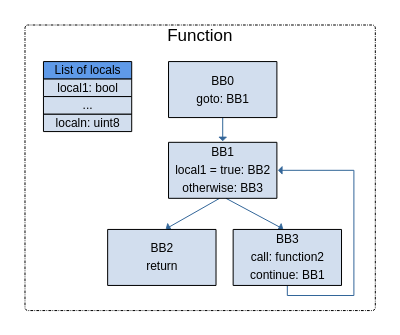
\includegraphics[width=.7\textwidth]{../diagrams/Function.png}
    \caption{
        Example of a functions internal control flow.
        The statements of the basic blocks are omitted as they don't affect control flow.
        A function has a list of locals that are accessible on the stack.
        Each local has an associated type.
        Functions always start with the first basic block (BB0 in this case).
        This function either returns to the calling function in BB2
        or calls `funtion2' in BB3.
        When function2 returns, control flow continues in BB1.}
    \label{mir_fn}
\end{figure}

It is also important to know that each function has a separate MIR representation.
Calling other functions is an action done by a call-terminator.
They can direct control flow to a subroutine that is executed until a return-terminator is hit.
After that the calling function resumes execution at a previously defined basic block.
An important note is that the functions in a call are referenced by name and not with an edge in the graph (this results in the separate MIR representation for each function).
This approach ensures that recursive function calls are kept simple.

Besides the specific kinds of statements and terminators, this is the general concept for the MIR graph.
A more detailed view would be of little help since it would get very close to the actual implementation.
Implementation details, however, are frequently changing;
In fact during this work it changed multiple times breaking the code.
A circumstance that is communicated by the compiler team and needed because a too stable API would restrain the compiler development process.


\section{Translation}
\label{app_trans}
After we saw how the MIR graph is structured, we can try to find a translation to Petri-Nets. This will include some more details and edge case we have to consider.

\subsection{Entry Point}
The will start with the most abstract view on our translation: the whole program.
A program is something that typically has a beginning end an ending.
We can model this with a \textbf{program start} and an \textbf{program end} place that every program has.
Depending on the program they are interconnected somehow.
The sole exception are programs with a diverging main function -- where the main function ends in an endless loop.
In this case start und end place will not be connected, but an unconnected end place does not harm either.
In rust a second end place for panics -- the \textbf{panic end} place -- is a helpful addition.
This place will be marked then the program terminated unsuccessfully after a panic was raised.
A circumstance that might be helpful to distinguishing in verification runs.
Finally the program start place needs to be marked with a token.
We will later see that this token also indicates the first statement to execute and that it virtually moves from statement to statement acting like a program counter (even though petri net tokens do not move semantically but rather be consumed and produced).

Although these are all the basic features shared by every program, we still have to look a little closer on the semantics of the program start place.
This place is a bit ambiguous since, in practice, the main function is not wat is executed first.
Usually programs have a `runtime' that is initialized before main() is called.
These setup static memory and initialize language specific features, among other things.
And even though low level languages like rust or c hove a small runtime, they still have one.
Now we have to decide if this runtime should be considered for Petri-Net translation.
After all it is part of the finally executed binary.
On the other hand it is platform dependent code that is independant from the actual program semantics.
And there is another problem in starting in the pre main code.
It turns out that the MIR for that part is not completely available in every compiler version.
It is possible to get the missing parts subsequently but it complicates the translation process unnecessarily.
Additionally, we previously argued for a platform independent approach already in chapter \ref{app_intercept}.
It would be inconsistent to detach from that agenda now.
So, because of these reasons we decided to skip the pre main() code and start translating programs with the actual main method.

\begin{figure}
    \centering
    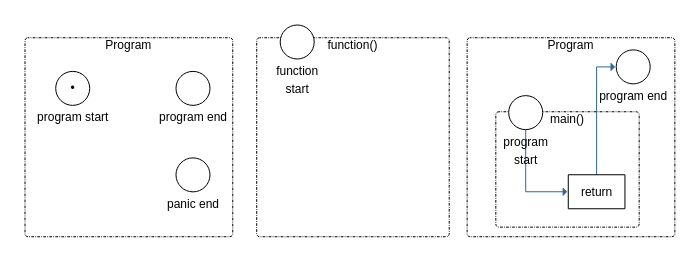
\includegraphics[width=.9\textwidth]{../diagrams/basic_program.png}
    \caption{
        Stubs for programs and functions, and a minimal terminating program.
        A program has a start and an end place.
        The start place holds a token, as program execution begins there.
        If a program terminates successfully the program end place is marked.
        A termination caused by a panic marks only the panic place.\\
        A function has a distinct starting place (it always starts at the first basic block).
        But there is no end place, as functions can be left by any terminator.\\
        The shortest possible (terminating) program has an empty main function.
        Program start place and main function start place are one and the same place.
        Empty functions have no basic block in MIR, so we have to add an artificial transition to leave the function.
    }
    \label{program_blocks_trans}
\end{figure}

\subsection{Functions}
After we modeled the important features of a program, we can look on the next important path that a program consists of.
Control flow wise these are functions.
As in most other imperative languages rust programs have a main function that wrap all its functionality (excluding the runtime as discussed in the previous section).
The main function can call other functions that inturn can call additional functions, and so on.
When executing a program the called functions are organized on a stack called `call stack'.
When a new function is entered a new stack frame is pushed on the stack including information like function arguments and local variables.
On leaving a function it is removed from the stack deallocating memory the frame occupied.

In MIR calling and returning from functions is done in a basic block terminator and can occur arbitrarily often.
Considering this behavior in a function model would be of no help, leaving just the start place as a feasible similarity between functions.
A function that is called always begins its execution there.
And it will always be identical to the start place of the first basic block.

So, from a modeling perspective functions are not the decisive abstraction.
But if we consider the translation process they get more important.
The rustc interface for MIR works per function.
This means that it is not possible (at least no obvious one) to get the MIR from a whole program but only from single functions.
A likely explanation for this design choice is that a lot of context information switches with functions.
For example every functions starts with basic block zero and increases the count for the following.
Local variables are also indexed with some of them having a special meaning.
The first being the functions return value followed by variables for all function arguments.
If we want to translate a program we have to keep this structure in mind.
In our implementation we have done this virtually by an own call stack.
We traverse the program function by function.
Every time we encounter a function call terminator we try to translate the called function and return wre we left if we are done.
On the new call the context is switched to the new variables and basic blocks, and the return semantics is stored.

However, this approach has some implications:
\begin{enumerate}
    \item If the same function is called multiple times in the program, it is also translated multiple times.
    Although, this can probably avoided with an intelligent function cache this approach is sufficient for a proof of concept.
    \item The far more extensive implication are the voided recursion capabilities.
    If we encounter a recursive function with this strategie, we will be trapt in an endless loop.
\end{enumerate}
Actually recursion is a feature that can never be achieved with low-level Petri-Nets, as it data model cannot be mapped correctly.
How often a recursive function is called depends on the data it is called with and cannot be known at compile time.
In normal program execution functions are just pushed on a new stack frame until it is resolved (the base case is called for all recursive calls) or the stack overflows.
Most relevant programs will be still executable.
But we cannot model this stack like behavior in low-level Petri-Nets because we cannot get additional memory.
All memory we have is that we know of at compile time.
And we cannot reuse the places of a function for different recursion levels as we can not distinguish the tokens from the recursion levels.
We could just remodel each recursion level again and again to a fixed recursion level.
However, this would impact the verification results, since a property might change for programs with different maximum recursion depths.

A solution to this problem can be high-level petri nets, where we can distinguish between tokens.
There we could reuse places from the same function by annotating tokens with the corresponding recursion level.
We won't go into detail of this approach, though, since this work is based on the low-level semantics.
We will just have to accept that we cannot translate recursive functions for the time being.

\subsection{Memory}
To translate a rust program we cannot focus only on flow.
We also need a valid representation of data.
Unfortunately, as mentioned before, data is complicated to model in low-level petri nets.
With only the concept of bare tokens, we can only model finite memory space and even if we do, modeling every state of every possible variable would bloat our net terribly.

To stay in the realm of low-level nets we have need to abstract from variable states.
In principle a Petri-Net place already is something that holds data: a set of tokens.
If we interpret a place as a memory location and a token is data, though we loose a lot of information, however, we still can analyse the program flow.
Additionally, this representation resonates well with a possible high-level extension where the token can be annotated with the current value of a variable.
So, to keep it simple we represent a memory location as a single place with a single token.
And we `read' from memory with a transition that consumes the token, while also producing a token.

Now in many programing language there are different concepts of memory that behave differently, and rust is no exception.
Basically we can distinguish between four different concepts:
\begin{enumerate}
    \item \textbf{Constant memory space}: The size of the constant space is known at compile time and the values of this space do not change during runtime (hence the name).
    The values of all constants are compiled into the executable and no computation is needed to get them.
    \item \textbf{Static memory space}: Like in the constant space, the size of the static memory space is known at compile time.
    The big difference is that data the static space can change during runtime.
    So during program startup, a fixed amount of memory is allocated and all static variables are initialized.
    Later they can be used rather similar as normal variables. With some rust specific constrains that we will not discuss here, as they are not important for Petri-Net translation.
    \item The \textbf{Stack}: there the size is known for each stack frame (function call).
    This is the combined size of all local variables a function needs for execution.
    If a function is called a now frame is pushed to the stack and if the function terminates the frame is removed.
    Since the last pushed frame will be the first to be removed (LiFo - Last in, first out), the stack can be managed without data fragmentation.
    \item The \textbf{Heap}: which is the place there every remaining memory goes.
    A dynamic variable, there the size cannot be known at compile time needs to allocate memory on demand at runtime.
    If the memory is not needed anymore, it will be deallocated and the again free space can be reused.
    Since both allocation and deallocation are on demand, this can introduce memory fragmentation, since the size of the holes is not uniform.
\end{enumerate}

The most prominent concept on the MIR layer is the stack.
Every part of the MIR is associated with a function which has a set of local variables (locals).
The current state of a local variable is changed by statements.
This includes the values the variable can be assigned to as well as information about variable liveness.
Each local starts in an uninitialized state until a statement is called to set it `storage live'.
A living variable can be assigned to arbitrary values (the type allows) as long as it is needed.
Afterwards a statement sets the variable `storage dead' to indicate that it will not be used again in this function call.
We can model this behavior with three Petri-Net places for each local: one place for the uninitialized state, one for the living state there the variable can be used and one for the dead state.
The first active state will be `uninitialized' so this one must be marked with a token initially.
The unique `storage live' and `storage dead' statements (which are special statements generated for the MIR) have to be called to traverse the three states.
They will consume a token from the previous state and produce one on the next.
This enforces that data access can only be done if a token is on the live place.
This way we can later verify if the liveness invariants are met.

Heap and static space is hidden behind local variables.
For example we can access a value on the heap by dereferencing a pointer we stored in a local.
In MIR this is done with a projection from a local that describes wich part of the local is used;
Which field of a struct, which index of an array or if we dereference the local for example.
This information is stored implicitly as MIR-place on which statements can operate.
Unfortunately this projects is hard to impossible to model.
Especially pointer dereferencing is a problem since the memory model is handled by the operating system at runtime.
But for all these projections the source -- the initial local -- is known.
If we use a projection in a statement we can interpret this as an access to the initial local.
Again we loose some information here in exchange for a manageable design.

What is much easier to model is the space for constant variables.
They behavior is close to locals that live for the entire runtime.
So they do not need any uninitialized or dead place, just a place that represents the current value.
In fact we can model the whole constant space as a single Petri-Net place, where every access is done with different transitions.
Where is no data manipulation anyway.
And again this approch resonates well with a possible high-level petri net extension where every accessing transition produces token with the corresponding constant values.

In conclusion we need two models for memory access: a a set of place for each local variable with uninitialized, live, and dead place, and a single place that represents the whole constant memory space.
Memory is accessed and modified in statements and if we have to handle heap space we can hide this behind an access of a local variable which is projected to other memory space that we are unable to control (or model).
Before take a deeper look on the memory using statements next we will see how we can model the basic blocks that contains the statements.

\subsection{Basic Blocks}

\begin{verbatim}
- elements
    - function
        - can panic
        - can diverge
        - can be empty (in theorie)
    - basic blocks
    - statement
        - rvalues and operands
        - assign
        - etc
    - terminator
        - goto
        - switch int
        - call
        - etc
- panic handling
    - do not catch by other threads
    - distinguish between successful and unsuccessful termination
- which parts can or must be excluded from translation
    - std implementations
    - part between std::mutex and pthread mutex
- emulating features
    - missing mir parts
    - external libraries
    - intrinsics and platform specific behavior
    - mutexes
        - high level and low level interfaces
        - choosing high level
            - harder model checking for more general Mutexes
            - os independent
            - less elements need to be translated
                - smaller net
                - worse mapping
        - need to track associated locals

- joining the translations
    - joining basic elements
    - joining basic blocks
    - joining function calls
    - recursion limits
\end{verbatim}
\begin{figure}
    \centering
    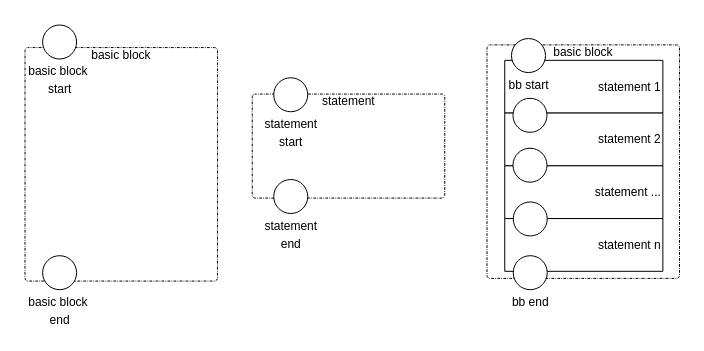
\includegraphics[width=.9\textwidth]{../diagrams/basic_blocks.png}
    \caption{
        The structure of basic blocks and statements.
        Basic blocks as well as statements have a distinct start and end place.
        The start place of the first statement is identical with the basic block start place.
        The same is true for the lasts statements end place and the basic block end.
        Also the end place of a leading statement is the start place of the following statement (illustrating the sequential nature of statements).
        Terminators are represented entirely by transitions that are not pictured here, as they are typically linking to other basic blocks.
    }
    \label{basic_block_trans}
\end{figure}

\section{Petri Net Representation}
\label{app_petri}
\begin{verbatim}
    - petri net formalism and format (high level? edge descriptions)
\end{verbatim}


\section{Model Checking}
\label{app_mc}
\begin{verbatim}
- many tools
- pnml as common representation language
    - finding tools on standard site
- lola integration (format of a petri net)
  - own format
- CTL formula
    - expected deadlocks (program end)
    - difference between deadlock in petri net and deadlock in program
        - try to stay analogous
    - difference between p = 0 and EF( p = 0 )
    - try to force witness paths
\end{verbatim}

\section{Test Programs}
\label{app_test}
\begin{verbatim}
- stay simple to prove concept
    - empty program
    - programs which cover the basic language features
    - program with a deadlock
    - similar program without a deadlock
\end{verbatim}

\section{Debugging}
\label{app_debug}
\begin{verbatim}
- dot file for small programms
- finding unconnected nodes
    - possible bug found
    - marking live places as result
    - uninitialized places still have to be marked
      (or removed entirely)
- witness path
    - reducing the complicated net to witness path nodes 
      and its neighbors
\end{verbatim}
\chapter{Result}
\label{results}
Having a concept on how to translate a rust program into a Petri-Net, we can now inspect the actual results.
\section{Translation target}
\begin{figure}
  \centering
  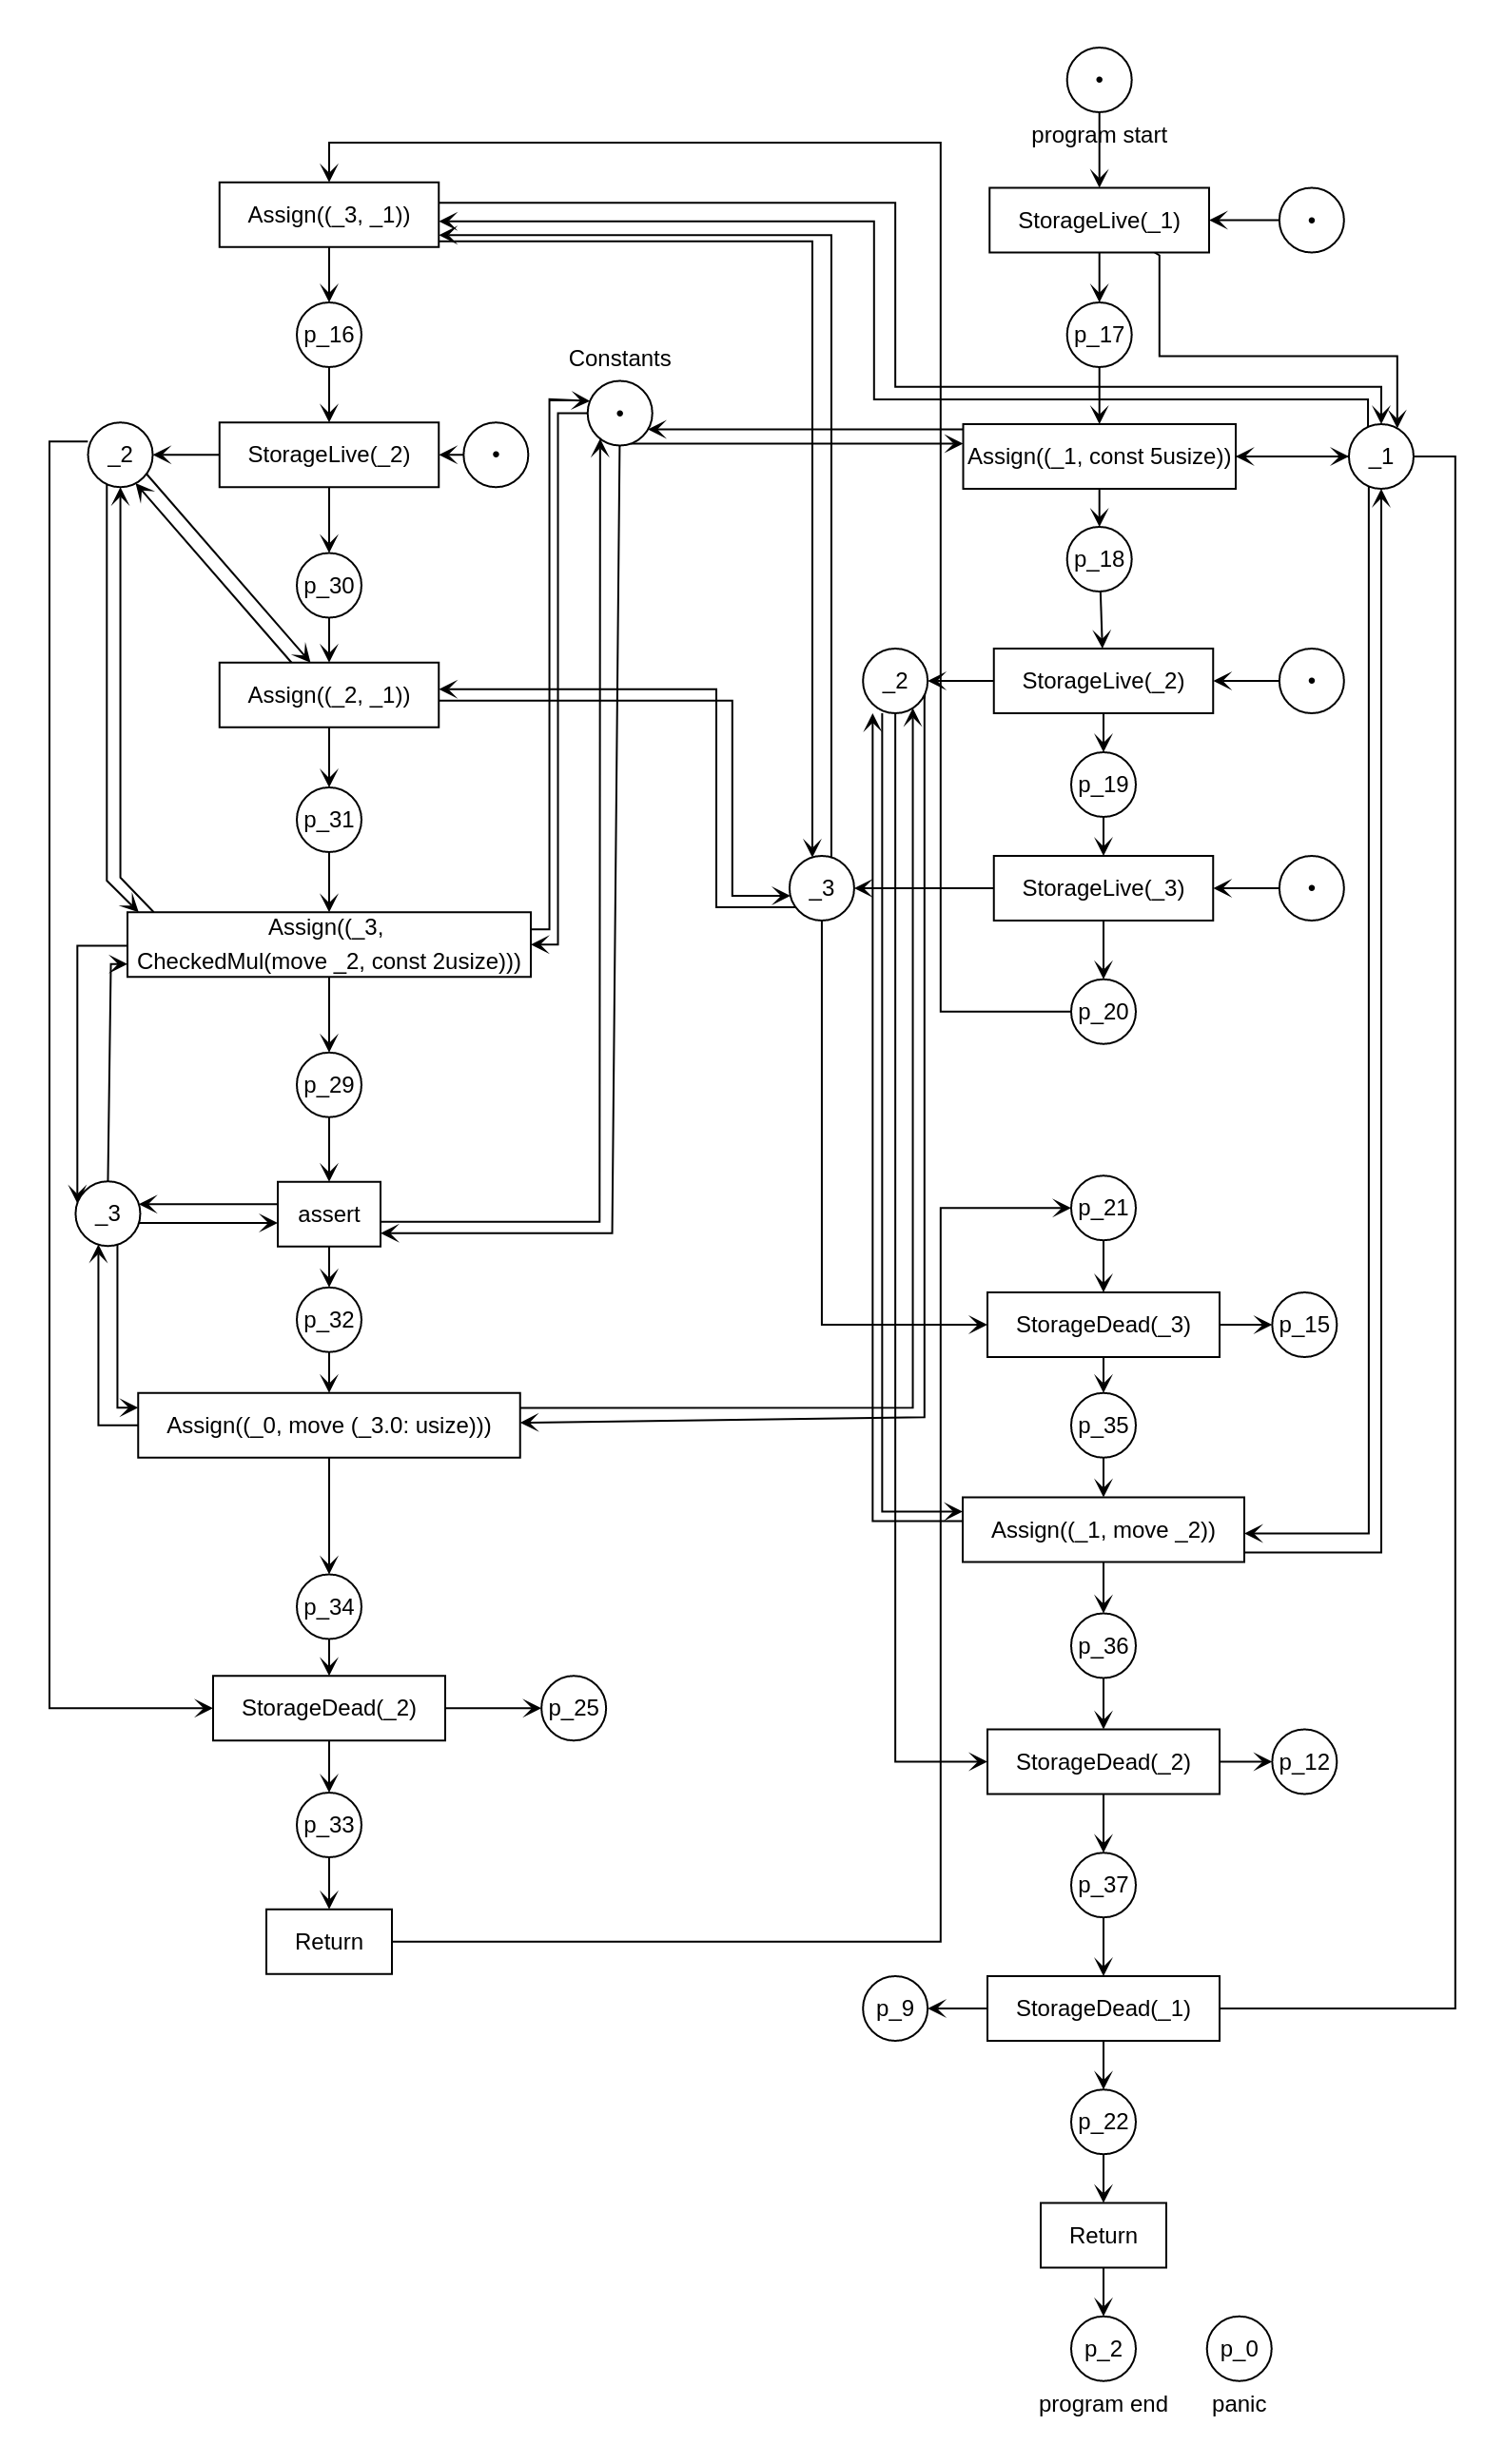
\includegraphics[width=0.9\textwidth]{../diagrams/FunctionCallNet.png}
  \caption{Translated Petr-net}
  \label{function_call_net}
\end{figure}
In figure \ref{function_call_net} we can see the generated net for the function call program \ref{function_call_program} from the last chapter (since this is small enough to show and big enough to not be trivial).
This is the true data that was produced for the dot target so we cannot immediately see the virtual boundaries for statements basic blocks and functions.
To make the structure more clear the nodes where rearranged so that the called function is on the left and the main function on the right.
The initialized places of the locals where renamed to show their name (locals are scoped by functions so their names are not unique).

We can see a path from program start to program end;
The panic place is unconnected because the program cannot panic.
Local life cycles are also visible as a single edged path from marked uninitialized place to unmarked dead places.
Variable manipulation always has parallel incoming and an outgoing edges.
On a closer look we can see that local $\_3$ of the called function has no initializing and uninitializing statements.
This is actually a correct representation of the MIR graph:
for some reason the storage statements are not generated for some lvalues (in this case the lvalue from checked multiplications).
If this is expected behavior is not known at the time of writing;
A bug report \cite has yet to be solved.
Unfortunately this behavior introduces an unintended deadlock into our translation since depending transitions can only fire if the initialized places where previously marked.
To use the net for verification we have to work around this issue until it is fixed (or until the cause is modeled correctly).
Te be able to continue testing simply all initialized place where marked.
This way the involved transitions can fire, but only if the previous transition produced a token on the connecting place (the program counter place). 
An additional taken will also remain on the initialized places even after the storage dead transition fired.
However execution flow, again, will not be affected because of the program counter places.

A second detail that the net shows is that the function call transition is implicit;
The last statement of the main functions first basic block is directly connected to the first statement of the callees first basic block.
This is an implementation detail of the translator.
Since our model currently always inlines function calls (it generates a separate net for every call), these are entirely sequential.
That means a missing transition does not harm.
If previously translated functions shall be reused though, this issue needs rework.
But to be able to skip inlining we need high level semantics anyway.

An additional issue that can come to attention is the missing cleanup ptah of the assert terminator.
This is the path that would lead to a panic.
Logically the assert is inserted because the preceding checked multiplication can overflow, which is undefined behavior and by default should panic in rust semantics.
This particular program cannot fail at this point, since the involved variables are constant and small enough to be multiplied.
If this is the reason why the panic path is not generated (or optimized away) in the MIR representation however, shall be a question for the rust compiler team.

\section{Verification results}
\begin{figure}
  \centering
  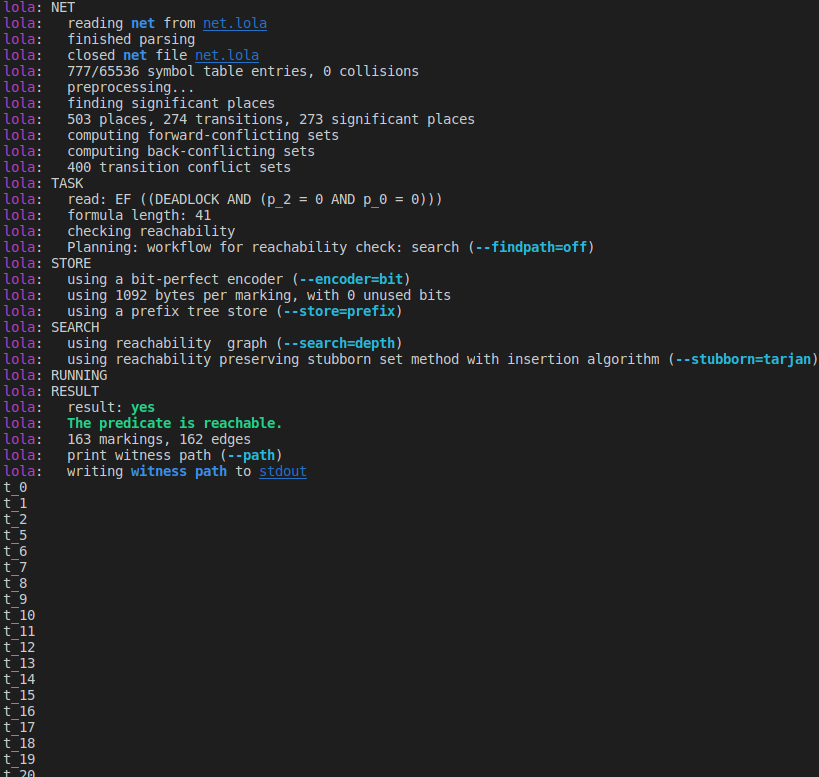
\includegraphics[width=1\textwidth]{./pictures/lola_output.png}
  \caption{LoLa output}
  \label{lola_output}
\end{figure}
Of course we want to use our translation further for verification.
Using our formula on the deadlock program from listing \ref{deadlock_program}, LoLa does find a deadlock and can produce a witness path as shown in figure \ref{lola_output}.
In contrast, if we remove the last line of the program, no deadlock is detected.
But, following the witness path does indeed lead to the transitions that are involved in the mutex emulation (the mutex place is empty causing involved transitions to be dead).
Earlier tests have also shown that the mutex emulation is necessary to produce deadlocks.
Without the information on where and how execution should be blocked, the translation process cannot infer this behavior.
This is a general problem for blocking behavior by external cause.

At this point it might be adequate to add that active waiting (looping until a guard has an expected value) is not a deadlock and also would not be detected with this approach.
However, it is likely that a another formula can be found that verifies that leaving the waiting section is always possible.
But again this most likely would require to consider the values that variables can hold.

\section{Discussion}
The results show that our basic approach can be used to verify some basic properties.
And even though the state of the translation is nowhere near productive use there are still some lessons that can be learned that we can discuss.
\subsection{The Model}
The main draw back that followed us for the entire process is the abstraction of data in low-level petri nets.
The advantages of the low-level model not only is the reduced complexity and higher verification performance, it can also produce stricter assertions.
Additionally, our particular model most likely can exploit a petri-net property called safety.
If we overlook the work around we discussed for compensating the missing storage-statements, the token count on every place cannot exceed a maximum of one.
One obvious use for that property is the state encoding for every place, which can be done with a single bit this way.
This might be helpful for very large programs with lots of places.

The greatest disadvantage of low level Petri-Nets is the reduced expressivness of data.
While flow related properties are easy to model with simple tokens, as soon as we enter the realm of data related properties, we have to make compromises.
The approach we took models every interaction with data but we cannot facilitate their set of possible values for verification tasks.
Another problem is that no moving data is modeled.
If a previously initialized local becomes part of another local (like a field of a struct) we completely loose this information in our translation.
Although, we can probably exploit rusts strict borrow checking and aliasing rules to model a much closer relation between data,
both locals are generated independently with their own places and life cycle.
An improvement for example for a move of a value from one local to another (which is encoded in MIR), is to connect the places with a transition right away.

Another disadvantage of our current model is the inlining of functions.
If a program calls the same function at different places a separat instance will be inserted at every call site.
This not only makes the net larger, it also causes the translation to diverge in recursive functions.

A solution for most of these problems might be high-level Petri-Nets where we can model data verbosely.
With them we could properly model data and detach function calls from the call site.
Only the cost for verification performance remains unknown at the moment.
Some problems, on the other hand, cannot be solved this way.
For example, program parts that are not represented by MIR (like foreign functions and compiler intrinsics) cannot be translated and have to be emulated.
Also information on blocking behavior is needed to model deadlocks appropriately.
For mutexes we again worked around this issue with emulation.
Additional blocking functionality (like waiting threads) have to be emulated separately.

\subsection{Verification}
The ability to discover deadlocks is already a useful property for model checking.
But our model is not restricted to this single property.
An easy addition is to check if the panic state is reachable.
Since increased complexity also increase the likelihood of operation that can panic this might be of limited use;
Unless variable data can be respected.
However, more complex properties could deal with conditional reachability.
For example if a function can be reached from a particular program state.
Or if every execution of a program eventually visits a function or statement.
But then again, our statements would be much stronger if we could consider if we consider data.

% !TEX root = ../main.tex
\chapter{Conclusion}
\label{conclusion}
The main goal of this work was finding a mapping from rust programs to Petri-Nets.
A translated net then was intended to be used in a model checker to find deadlocks.

To reach that goal we searched for a suitable representation for rust programs and developed a set of rules to translate that representation into Petri-Nets.
We did this for the basic components and constructed a complete model out of that components.
Because some important flow related information -- like blocking execution -- is hard to detect with our approach, we also added an emulation for rust mutex locks.
And finally we tested if a simple test program can be translated and verified with a model checker to find the expected deadlock.

An analysis of our translation showed that our data model is very abstract and probably can be further improved.
However, the model of program flow seems to be close to the execution semantics of rust programs.
Our test showed the expected behavior, but complex programs where not tested because the implementation does not cover all necessary features.
Yet, the general approch seems to be applicable and can be refined further to deal with complex scenarios.

% !TEX root = ../main.tex
\chapter{Future Work}
\bibliography{IEEEabrv,literature}
\bibliographystyle{IEEEtran}

%% Zum Abschluss die Eidesstattliche Versicherung
\newpage
\thispagestyle{empty}
\label{EidesstattlicheVersicherung}
\vspace*{8cm}% Abstand zum oberen Seitenrand
{\parindent 0pt
    \textbf{\Huge{Eidesstattliche Versicherung}}\vspace{10mm}\\
    Hiermit versichere ich, dass ich die vorliegende Arbeit selbstständig verfasst und keine anderen als die angegebenen Quellen und Hilfsmittel benutzt habe, alle Ausführungen, die anderen Schriften wörtlich oder sinngemäß entnommen wurden, kenntlich gemacht sind und die Arbeit in gleicher oder ähnlicher Fassung noch nicht Bestandteil einer Studien- oder Prüfungsleistung war.
    \\[2cm]}
Rostock, 02. März 2018
\\[3cm]
\rule{6cm}{0.5pt}\\
\parbox[l][1cm][c]{6cm}{\hfill\name\hfill\vbox{}}

\end{document}
